\chapter{Methods\label{chap:Methods}}
% notes: Previous research (discussed in Chapter~\ref{chap:Bkgd}) reveals that virtually any XXX can impact speech perception, and various prosodic dimensions vary with dialect.  Also one limitation of using \psola{} for resynthesis is the limitation of 50Hz / 20ms
%TODO: explain why I used syllablewise duration

\section{The \ac{pn/nc} corpus}
Stimuli for the experiments described here were a subset of the \ac{ieee} “Harvard” sentences \citep{HarvardSents} drawn from the \ac{pn/nc} corpus \citep{xxx}.  The sentences in the \ac{pn/nc} corpus were selected based on absence of alliteration or rhyming, avoidance of focus/contrast readings, and lack of marked locutions; The full list of sentences used is given in Appendix~\ref{apx:HarvardSents}.  

Based on within-dialect intelligibility scores from \citet{McCloyEtAl2013}, three talkers were chosen for the present experiments, herein referred to as talkers \ac{a}, \ac{b}, and \ac{c}.  These talkers were selected because, as a group, the Pacific Northwest male talkers exhibited the largest spread in inherent intelligibility in the corpus, and those three talkers formed the endpoints and midpoint of that group, with talker \ac{a} being the most intelligible and talker \ac{c} the least intelligible (cf. Figure~\ref{fig:dotchart}).

\begin{figure}
	\begin{centering}
	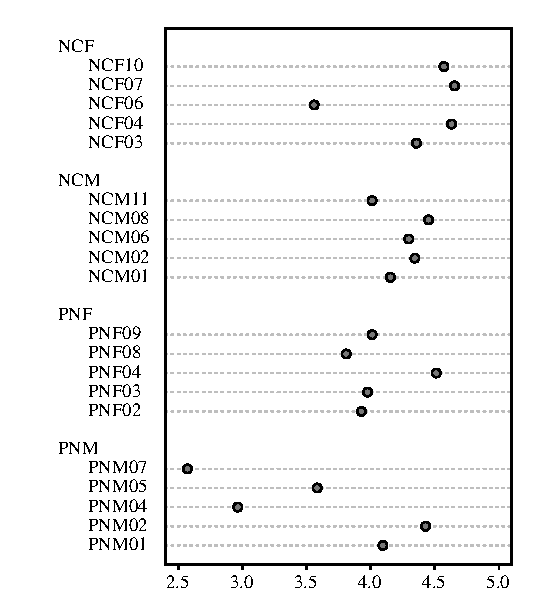
\includegraphics{figures/dotchart.eps}
	\caption[Intelligibility of talkers used to make the stimuli]{By-talker mean keywords correct (across dialect-matched listeners) in speech-shaped noise at +2 dB \ac{snr} (adapted from \citet{McCloyEtAl2013}).\label{fig:dotchart}}
	\end{centering}
\end{figure}

\section{Stimulus design\label{sec:StimDesign}}
Stimuli underwent prosodic replacement via \psola{} resynthesis, as implemented in Praat \citep{praat}.

Duration was matched at the syllable level.  Syllable boundaries were determined based primarily on local minima in the intensity contour of the sentence, with reference to inflection points in the intensity contour or waveform envelope, or to aspects of waveform or spectrogram morphology, when intensity contour minima were absent from the syllable transition region (see Script~\ref{scr:SyllIntens}).  This method was chosen over two competing methods — marking only periodic/aperiodic transitions, or marking all phonemic\slsh{}segmental boundaries — because both of those methods suffer from inter-talker differences in the number of units in a given sentence, whereas virtually all sentences in the corpus showed inter-talker agreement on number of syllables.

Automatically detected glottal pulses were hand-corrected, and pitch values were derived from the intervals between pulses (see Script~\ref{scr:PulseCor}).  In a small number of stimuli containing creaky voicing, alternating short-and-long inter-pulse intervals were marked, rather than omitting alternating pulses (which would have effectively halved the pitch).  This was done for the purpose of better resynthesis.  The temporal locations of donor pitch points were shifted via dynamic time warping prior to being mapped onto the target signal.

Intensity was altered by first multiplying the signal by the difference of the maximum intensity and the inverted intensity contour (see Figure~xxx), then multiplying the resulting signal by the intensity contour of the replacement prosody and scaling as needed to achieve the desired \ac{rms} amplitude.  To do this, the donor intensity contour first underwent dynamic time warping to match the durational patterns of the target signal (see Script~\ref{scr:Psola}).

  

% Why \ac{psola}?  Brief comparison of different methods for manipulating duration.  Malah1979 ("linearly combining adjacent intervals of speech to avoid major discontinuities in the waveform"), MoulinesCharpentier1990 (\ac{psola}).  Relate to the studies that used them: PichenyEtAl1989 (Malah method), UchanskiEtAl1996 (segment-by-segment time scaling), LiuZeng2006 (adding silences, "uniform scaling" = \ac{psola}?).  Cf KrauseBraida2002, KrauseBraida2004.

\section{final stimulus creation}	
	\begin{itm}
		\item{\ac{rms} normalization}
		\item{create speech shaped noise}
		\item{mix signal and noise — justify chosen \ac{snr}}
%		\item{discuss danger of doing \ac{snr} before \ac{rms} — target signal below threshold}
	\end{itm}


\section{experiment sessions}
% Rationale for how much training to do:  
% \citep{YonanSommers2000}: Trained talkerID on 4 talkers (2M2F) over 2 days.  Each day: 60 exposure trials, 40 trials training w/ feedback, 60 more exp, 40 more training, 80 test.  All phases were half high-context and half low-context sentences.  End of day 2: single words \& sentences in SNR -5,0,+5, half high- half low-context, half familiar talkers half novel, half male talkers half female.  Familiar/unfamiliar talkers were piloted to make sure they were equally intelligible generally, and to old vs young people.  RESULTS: young listeners near ceiling on talkerID both day1 and day2; old listeners 73\% and 76\%.  Training on sentence material did not aid on the single word task (same as NygaardPisoni1998).  There was a benefit of familiar talker for sentence materials, which was stronger at lower SNRs.  A similar pattern obtained for a second experiment with talker exposure instead of talkerID training.
% \citep{VanEngen2012}: Two 30-minute training sessions (64 sentences) with noise (either SSN, English 2-babble, Mandarin 2-babble) and feedback.  Posttest 1 familiar, 1 unfamiliar talker, half in English babble, half in mandarin.  Trained and tested at their HINT threshold -3dB (based on VanEngen2010) to avoid floor/ceiling.  Results: “(1) listeners were able to take advantage of target talker familiarity; (2) training with babble was more effective than SSN training; and (3) after babble training, listeners improved most in coping with the babble in which they were trained [English or Mandarin]. In general, the results show that processes related both to tuning in to speech targets and tuning out speech maskers can be improved with auditory training”

Stimuli were presented with a stationary gaussian masker noise, frequency shaped to match the long term spectral average of the corpus of stimuli, at 0 dB \ac{snr}.  This \ac{snr} was chosen to avoid ceiling and floor effects, based on a pilot study testing five \ac{snr}s ranging from −1 to +3 dB.  To ensure target audibility, the level of the speech was held constant at 67 dB \ac{spl} (dB \ac{rms} in a 6 cc coupler) and the masker noise was digitally added to the speech to achieve the desired \ac{snr}, yielding a final presentation level of approximately 70 dB \ac{spl}.  The noise extended past the beginning and end of the speech by 50 ms in each direction, and linear onset and offset ramps were applied to this excess noise to prevent clicks during stimulus playback.

The combined speech-and-noise signal was presented in a sound-insulated booth over closed-back supra-aural headphones (Sennheiser HD 25–1 II).  Listeners were instructed to repeat each sentence they heard, to give partial answers when they only heard some words, and to guess when they were unsure.  Trials were scored 0–5 on keywords correct during the task.  An audio recording was made of listener responses, and scoring uncertainties were resolved offline by a second researcher.  Talker-sentence-\ac{snr} assignments were random and unique for each listener, with the following constraints: (a) each listener heard each talker an equal number of times; (b) each listener heard each sentence only once.

SUBJECTS
\begin{itm}
	\item{number of listeners}
	\item{hearing test}
	\item{dialect controls}
	\item{demographics: age, gender, ethnicity, geography}
	\item{English native; other languages?}
\end{itm}

\section{data analysis}
\begin{itm}
	\item{mixed effects models?}
\end{itm}
